% =====================================================================
% Template Laporan Tugas — Workshop Deep Learning (Teknik Telekomunikasi ITERA)
% Studi Ablasi RNN, LSTM, GRU vs ANN untuk Prediksi Trafik Seluler
%
% Format IEEE conference dua kolom, MAKSIMAL 6 HALAMAN termasuk referensi.
% Compile: pdflatex main && bibtex main && pdflatex main && pdflatex main
%          (atau: latexmk -pdf main.tex). Bisa juga diunggah ke Overleaf.
%
% Teks bertanda [ ... ] adalah petunjuk: HAPUS dan ganti dengan isi kalian.
% =====================================================================
\documentclass[conference,a4paper]{IEEEtran}
\IEEEoverridecommandlockouts

\usepackage[indonesian]{babel}
\usepackage[utf8]{inputenc}
\usepackage[T1]{fontenc}
\usepackage{cite}
\usepackage{amsmath,amssymb}
\usepackage{graphicx}
\usepackage{booktabs}
\usepackage{siunitx}
\usepackage{xcolor}
\usepackage[hidelinks]{hyperref}
\graphicspath{{gambar/}}

% Penanda petunjuk (hapus pemakaiannya di versi akhir)
\newcommand{\petunjuk}[1]{\textcolor{gray}{[#1]}}

\begin{document}

\title{Studi Ablasi RNN, LSTM, dan GRU dibandingkan ANN untuk Prediksi Trafik Seluler Kota Milan}

% Satu blok per anggota (maks. 3). Hapus blok yang tidak dipakai.
\author{
\IEEEauthorblockN{Vaulina Fatrisia Siburian}
\IEEEauthorblockA{NIM 124400011\\
Teknik Telekomunikasi, ITERA\\
vaulina.124400011@student.itera.ac.id}
}

\maketitle

\begin{abstract}
Prediksi trafik seluler penting untuk memahami perubahan penggunaan jaringan dari waktu ke waktu. Penelitian ini membandingkan Artificial Neural Network (ANN), Recurrent Neural Network (RNN), Long Short-Term Memory (LSTM), dan Gated Recurrent Unit (GRU) menggunakan dataset Telecom Italia di Kota Milan. Pengujian dilakukan pada lokasi Duomo dan Navigli (Darsena). Studi ablasi mencakup ukuran jendela waktu, jumlah unit tersembunyi, jumlah lapisan, laju pembelajaran, kombinasi fitur, ukuran batch, dan dropout. Setiap konfigurasi dievaluasi menggunakan tiga seed. Pada lokasi Duomo, konfigurasi terbaik GRU menghasilkan test Mean Absolute Error (MAE) sebesar 220,3, dibandingkan dengan 270,7 untuk ANN, 224,5 untuk RNN, dan 245,6 untuk LSTM. Hasil ini menunjukkan bahwa GRU memperoleh kesalahan prediksi terendah di antara empat model pada pengujian tersebut. Pengujian di Navigli digunakan untuk mengamati kemampuan generalisasi model pada lokasi berbeda. Hasil eksperimen menunjukkan bahwa pemilihan model perlu mempertimbangkan karakteristik lokasi dan pola trafik pada periode tertentu, termasuk periode Natal.
\end{abstract}

\begin{IEEEkeywords}
prediksi trafik seluler, RNN, LSTM, GRU, studi ablasi
\end{IEEEkeywords}

% ---------------------------------------------------------------------
\section{Pendahuluan}

Peramalan trafik seluler diperlukan untuk membantu operator telekomunikasi memahami pola penggunaan jaringan dan merencanakan kapasitas jaringan. Trafik dapat berubah berdasarkan waktu dan lokasi sehingga diperlukan model yang mampu mempelajari pola dari data historis.

Artificial Neural Network (ANN) mempelajari hubungan antara masukan dan keluaran, sedangkan Recurrent Neural Network (RNN), Long Short-Term Memory (LSTM), dan Gated Recurrent Unit (GRU) dirancang untuk mempelajari pola berurutan pada data deret waktu. LSTM menggunakan mekanisme gerbang untuk membantu mempelajari ketergantungan jangka panjang \cite{hochreiter1997lstm}, sedangkan GRU menggunakan struktur gerbang yang berbeda \cite{cho2014gru}.

Studi ablasi dilakukan dengan mengubah faktor eksperimen untuk mengetahui pengaruhnya terhadap kinerja model. Kontribusi laporan ini meliputi perbandingan empat arsitektur model, evaluasi pengaruh parameter pelatihan dan fitur masukan, serta pengamatan kemampuan generalisasi model pada lokasi yang berbeda.


% ---------------------------------------------------------------------
\section{Data dan Metode}

\subsection{Dataset}
Empat arsitektur dibandingkan dalam penelitian ini. ANN digunakan sebagai model pembanding tanpa pemrosesan urutan secara rekuren. RNN memproses informasi berurutan, sedangkan LSTM dan GRU menggunakan mekanisme gerbang untuk membantu mempelajari ketergantungan temporal. Konfigurasi acuan menggunakan panjang jendela 24 jam dan horizon prediksi satu jam. Ukuran hidden, jumlah lapisan, fitur masukan, optimizer, laju pembelajaran, ukuran batch, dan pengaturan penghentian awal mengikuti nilai pada Tabel~\ref{tab:acuan}.


\begin{figure}[t]
  \centering
  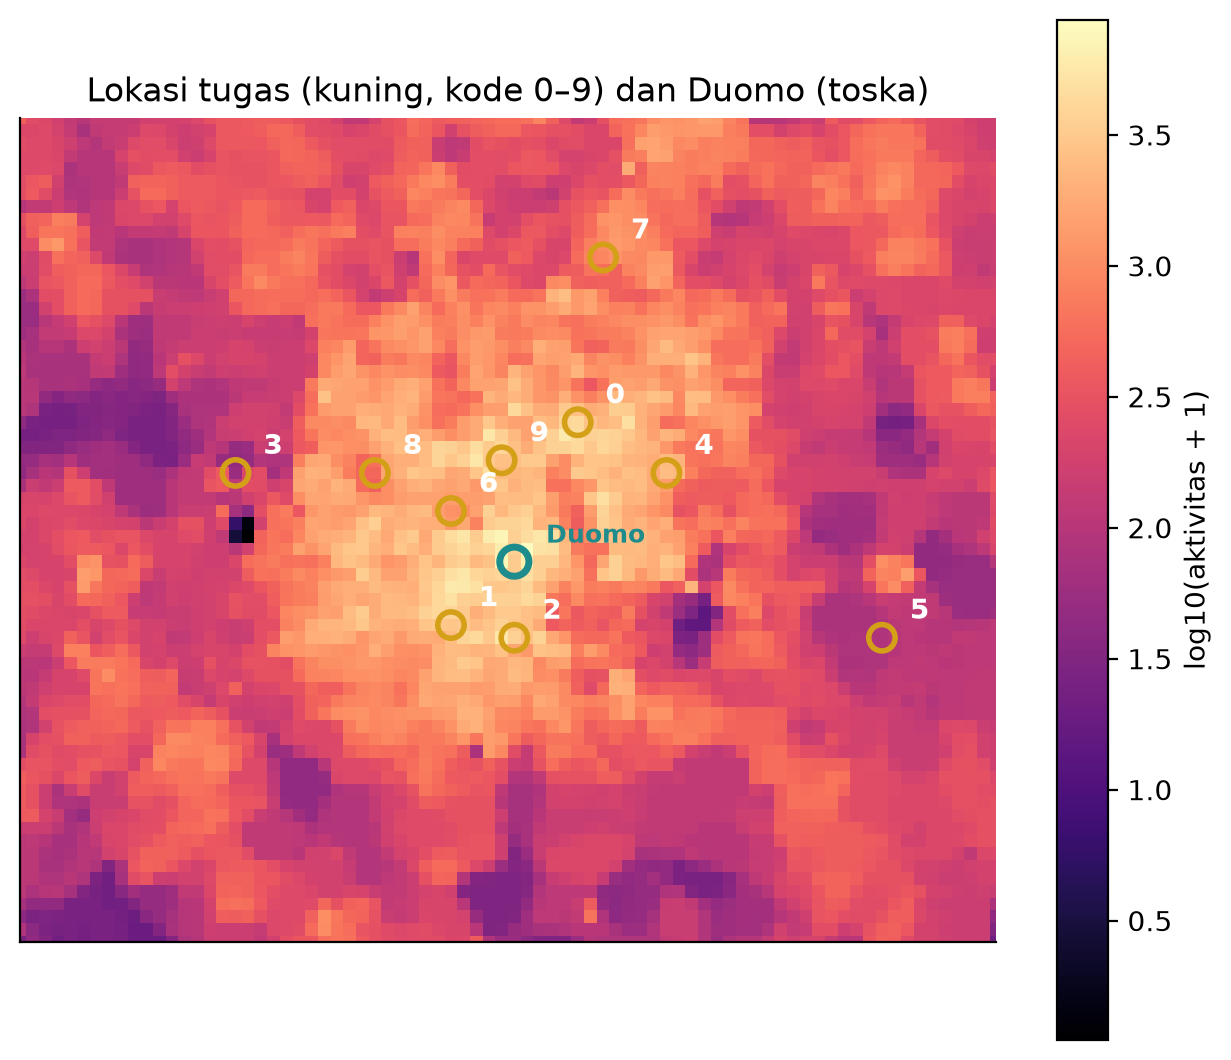
\includegraphics[width=0.85\linewidth]{peta_lokasi_tugas.png}
  \caption{Rata-rata aktivitas internet per kotak di Milan. Lingkaran kuning: lokasi tugas (kode 0--9); lingkaran toska: Duomo.}
  \label{fig:peta}
\end{figure}

\subsection{Pembagian Data dan Praproses}
Data dibagi berdasarkan urutan waktu menjadi data pelatihan (\textit{train}), validasi (\textit{validation}), pengujian (\textit{test}), dan periode khusus Natal. Standarisasi dilakukan menggunakan statistik yang dihitung dari data sebelum minggu validasi. Data kemudian disusun menggunakan metode jendela waktu (\textit{windowing}) untuk memprediksi trafik satu jam berikutnya. Data deret waktu tidak diacak karena urutan waktu merupakan bagian penting dari pola trafik. Pengacakan dapat menyebabkan data dari waktu mendatang tercampur dengan data masa lalu sehingga evaluasi tidak lagi mencerminkan kondisi prediksi yang sebenarnya.

\subsection{Model dan Konfigurasi Acuan}
Empat arsitektur model digunakan dalam penelitian ini, yaitu Artificial Neural Network (ANN), Recurrent Neural Network (RNN), Long Short-Term Memory (LSTM), dan Gated Recurrent Unit (GRU). ANN digunakan sebagai model pembanding untuk mempelajari hubungan antara masukan dan keluaran. RNN memproses data secara berurutan sehingga dapat mempelajari pola temporal. LSTM menggunakan mekanisme gerbang untuk membantu mempertahankan informasi dalam jangka panjang \cite{hochreiter1997lstm}, sedangkan GRU menggunakan mekanisme gerbang dengan struktur yang berbeda \cite{cho2014gru}. Konfigurasi acuan setiap model meliputi panjang jendela 24 jam dan horizon prediksi satu jam. Parameter lainnya, seperti ukuran *hidden*, jumlah lapisan, fitur masukan, dan pengaturan pelatihan, ditunjukkan pada Tabel~\ref{tab:acuan}.

\begin{table}[t]
  \centering
  \caption{Konfigurasi acuan}
  \label{tab:acuan}
  \begin{tabular}{@{}ll@{}}
    \toprule
    Hyperparameter & Nilai acuan \\
    \midrule
    Panjang jendela $W$ & 24 jam \\
    Horizon & 1 jam \\
    Ukuran hidden & ANN 32, RNN 68, LSTM 33, GRU 38 \\
    Jumlah lapisan & ANN 2, rekuren 1 \\
    Fitur & net, call, sms, jam, hari (7) \\
    Optimizer, \textit{learning rate} & Adam, $10^{-3}$ \\
    \textit{Batch size} & 64 \\
    \textit{Early stopping} & \textit{patience} 30, maks.\ 300 epoch \\
    \bottomrule
  \end{tabular}
\end{table}

\subsection{Protokol Ablasi dan Evaluasi}
Studi ablasi dilakukan dengan mengubah satu faktor pada setiap rangkaian eksperimen. Faktor yang diuji meliputi panjang jendela waktu (A1: 6, 12, 24, 48, dan 168 jam), ukuran *hidden* (A2: 16, 32, 64, dan 128), jumlah lapisan (A3: 1, 2, dan 3), laju pembelajaran (A4: \(10^{-4}\), \(10^{-3}\), dan \(10^{-2}\)), serta kombinasi fitur masukan (A5: net, net+call+sms, net+waktu, dan semua fitur). Dua faktor tambahan yang diuji adalah ukuran batch (B1: 16, 64, dan 256) serta *dropout* (B2: 0, 0,2, dan 0,5). Pengujian dilakukan untuk mengetahui pengaruh setiap faktor terhadap kinerja model. Setiap konfigurasi diuji menggunakan tiga *seed*, dan konfigurasi terbaik dipilih berdasarkan MAE validasi. Kinerja model dievaluasi menggunakan MAE, RMSE, dan MAPE pada skala asli. Eksperimen dijalankan menggunakan CPU dengan PyTorch versi 2.14.0+cpu, dengan total waktu pelatihan sekitar 207,5 menit.
% ---------------------------------------------------------------------
\section{Hasil}

\subsection{Baseline Naif dan Acuan}
Hasil baseline naif digunakan sebagai pembanding untuk mengetahui kemampuan model dalam memprediksi trafik. Pada lokasi Navigli (Darsena), baseline naif dengan menggunakan nilai trafik terakhir memperoleh MAE sebesar 272,0 pada data pengujian, sedangkan penggunaan nilai trafik pada hari sebelumnya menghasilkan MAE 342,3 dan nilai trafik pada minggu sebelumnya menghasilkan MAE 471,4. Hasil ini menunjukkan bahwa baseline naif dengan nilai terakhir memiliki kesalahan pengujian paling rendah di antara ketiga metode tersebut.
```latex
\subsection{Ablasi Wajib}

Ablasi dilakukan untuk mengamati pengaruh perubahan parameter terhadap kinerja model prediksi trafik seluler. Pengujian dibagi menjadi lima faktor utama, yaitu panjang jendela waktu (A1), ukuran \textit{hidden} (A2), jumlah lapisan (A3), laju pembelajaran (A4), dan kombinasi fitur masukan (A5). Hasil setiap faktor dianalisis menggunakan grafik pada folder \texttt{hasil/}. Konfigurasi terbaik dipilih berdasarkan MAE validasi terendah.

\subsubsection{A1: Panjang Jendela Waktu}

Pengujian A1 dilakukan menggunakan panjang jendela waktu ($W$) sebesar 6, 12, 24, 48, dan 168 jam. Pengujian ini bertujuan untuk mengetahui pengaruh banyaknya data historis yang digunakan terhadap kesalahan prediksi trafik seluler.

\begin{figure}[t]
    \centering
    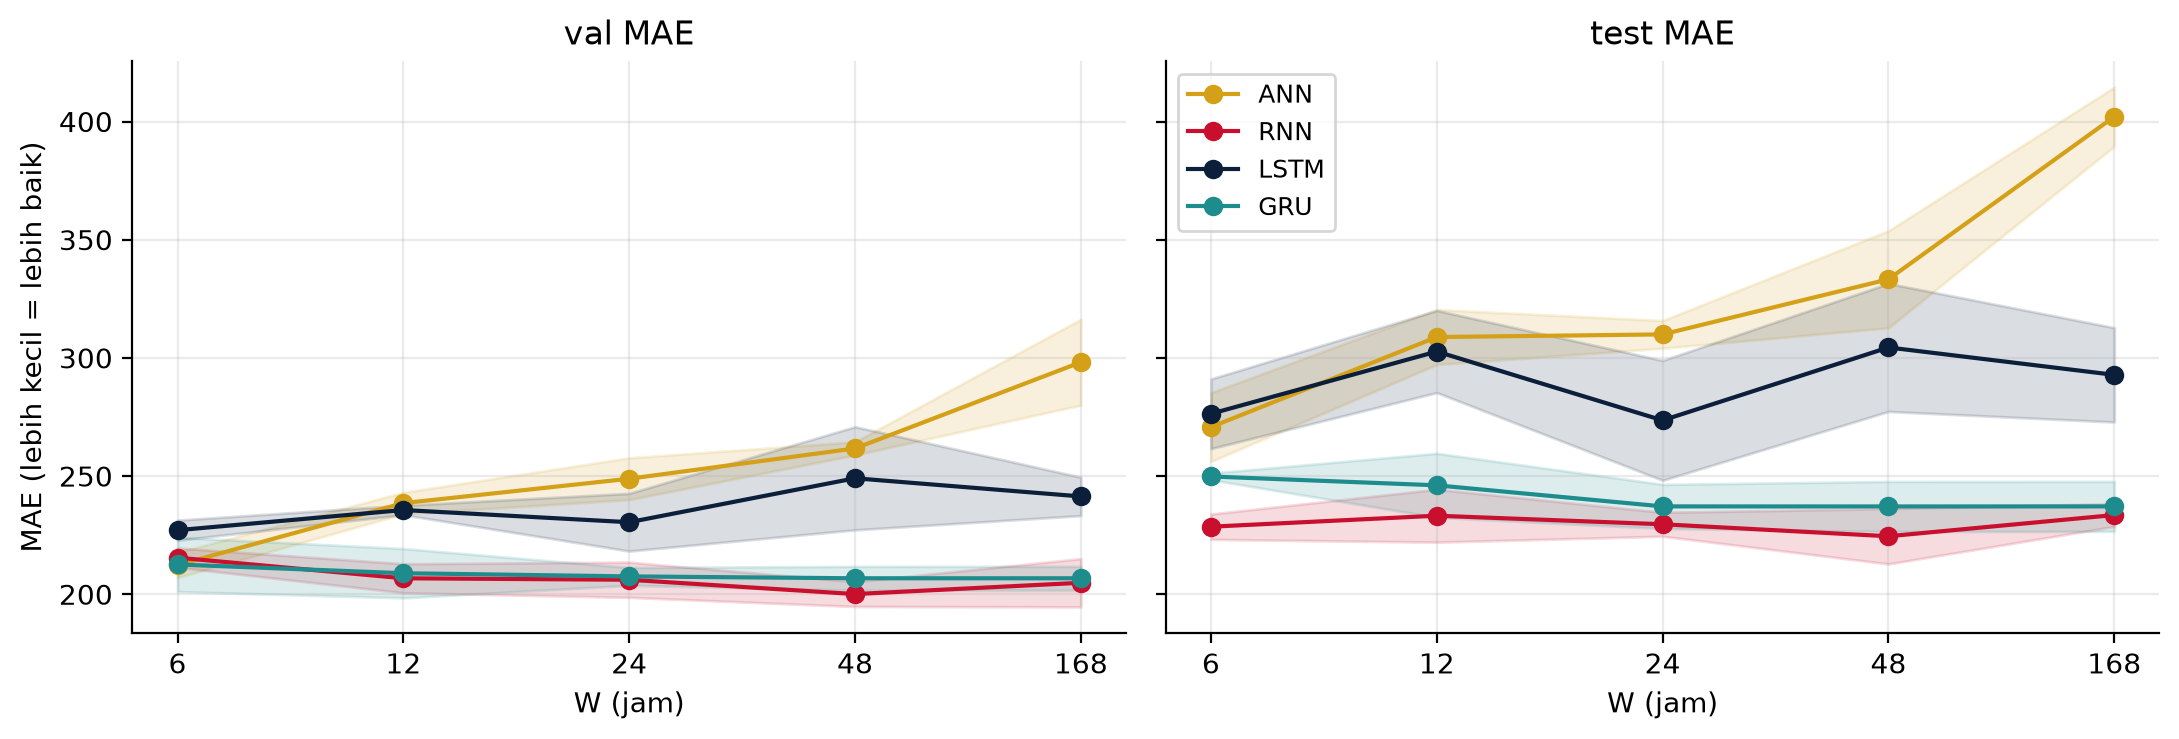
\includegraphics[width=\linewidth]{hasil/A1_W.png}
    \caption{Pengaruh panjang jendela waktu terhadap MAE empat model.}
    \label{fig:a1}
\end{figure}

Berdasarkan Gambar~\ref{fig:a1}, perubahan panjang jendela waktu menghasilkan respons yang berbeda pada setiap model. ANN menunjukkan kecenderungan peningkatan MAE seiring bertambahnya panjang jendela, terutama pada 48 dan 168 jam. RNN mengalami fluktuasi MAE, dengan penurunan pada jendela 24 jam dan kenaikan kembali pada 48 jam. Sementara itu, LSTM menunjukkan MAE yang relatif rendah dan stabil pada sebagian besar pengujian. GRU juga memiliki MAE yang relatif stabil, terutama pada jendela 24 hingga 168 jam. Berdasarkan grafik, LSTM mencapai MAE terendah pada jendela 48 jam, sedangkan GRU menunjukkan kinerja yang konsisten pada beberapa panjang jendela. Hasil ini menunjukkan bahwa penggunaan data historis yang lebih panjang tidak selalu menghasilkan prediksi yang lebih akurat. Oleh karena itu, pemilihan panjang jendela waktu perlu disesuaikan dengan karakteristik dan hasil evaluasi masing-masing model.

\subsubsection{A2: Ukuran Hidden}

Pengujian A2 dilakukan menggunakan ukuran \textit{hidden} sebesar 16, 32, 64, dan 128. Pengujian ini bertujuan untuk mengetahui pengaruh jumlah unit pada lapisan tersembunyi terhadap kinerja model prediksi trafik seluler.

\begin{figure}[t]
    \centering
    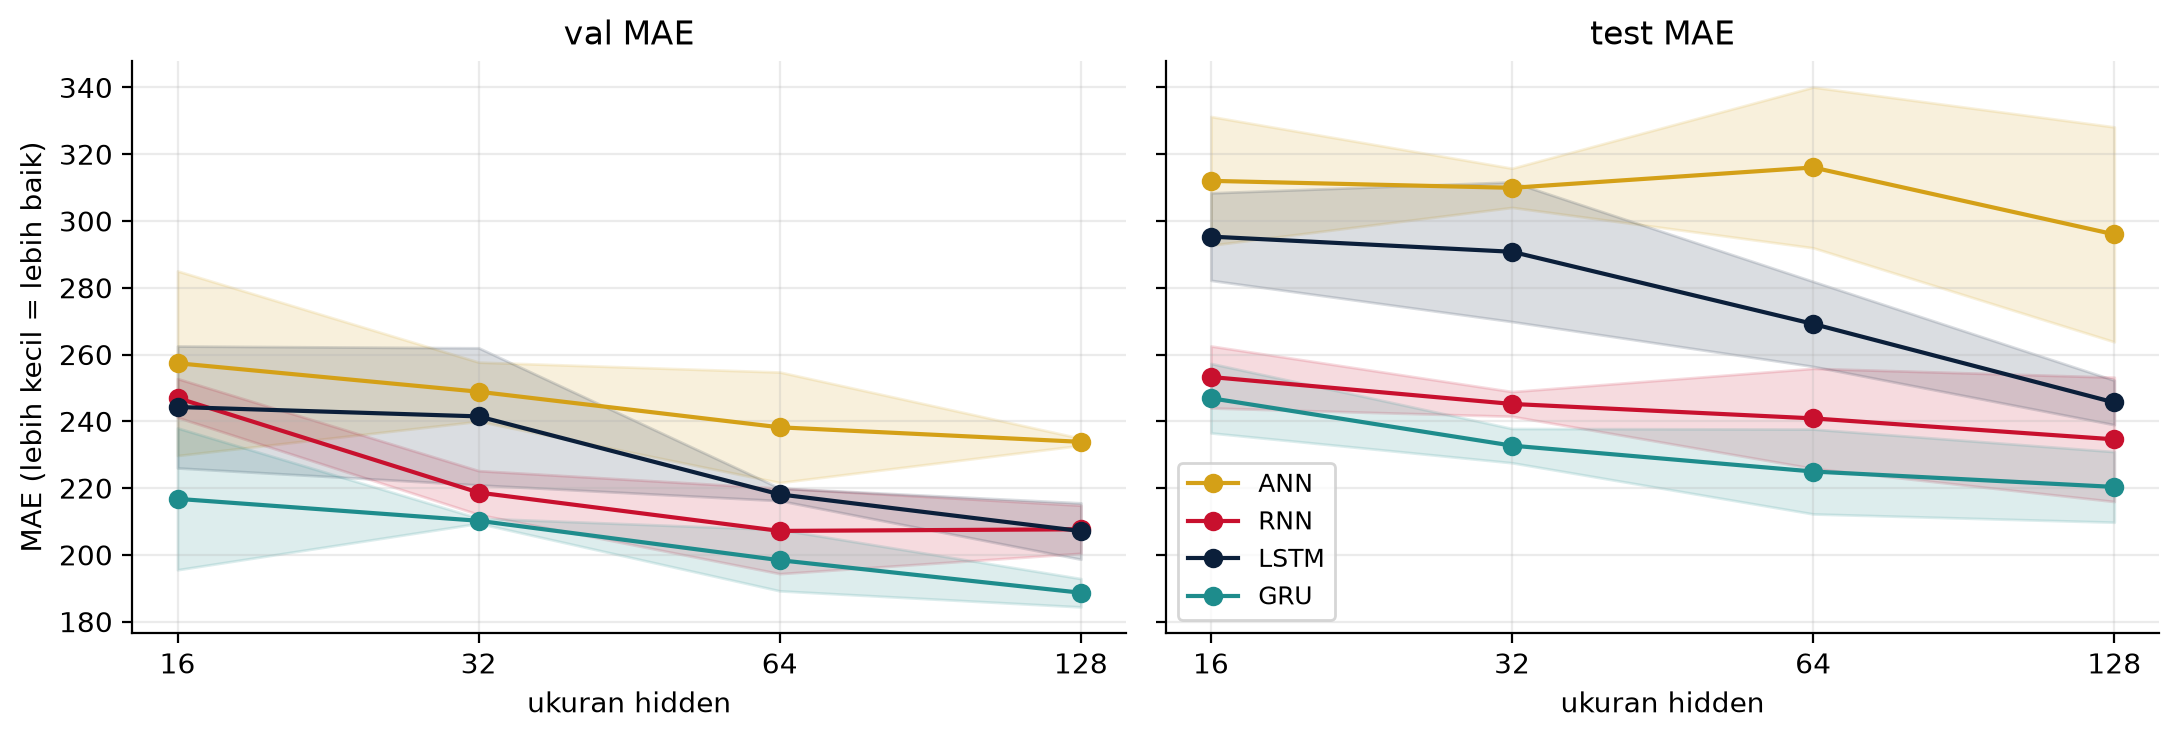
\includegraphics[width=\linewidth]{hasil/A2_hidden.png}
    \caption{Pengaruh ukuran hidden terhadap MAE pada data validasi dan pengujian.}
    \label{fig:a2}
\end{figure}

Berdasarkan hasil pengujian pada Gambar~\ref{fig:a2}, perubahan ukuran \textit{hidden} memengaruhi kinerja setiap model. Pada data validasi, ANN menunjukkan penurunan MAE secara bertahap seiring bertambahnya ukuran \textit{hidden}. RNN, LSTM, dan GRU juga cenderung mengalami penurunan MAE. Pada data pengujian, ANN menunjukkan perubahan MAE yang berfluktuasi, sedangkan RNN dan LSTM mengalami penurunan MAE ketika ukuran \textit{hidden} diperbesar. GRU menunjukkan MAE terendah pada ukuran \textit{hidden} 128, baik pada data validasi maupun pengujian. Hasil ini menunjukkan bahwa peningkatan ukuran \textit{hidden} dapat membantu mengurangi kesalahan prediksi, tetapi pengaruhnya berbeda pada setiap model. Oleh karena itu, pemilihan ukuran \textit{hidden} perlu mempertimbangkan hasil evaluasi validasi dan pengujian.
\subsubsection{A3: Jumlah Lapisan}

Pengujian A3 dilakukan menggunakan 1, 2, dan 3 lapisan untuk mengetahui pengaruh kedalaman model terhadap kinerja prediksi trafik seluler.

\begin{figure}[t]
    \centering
    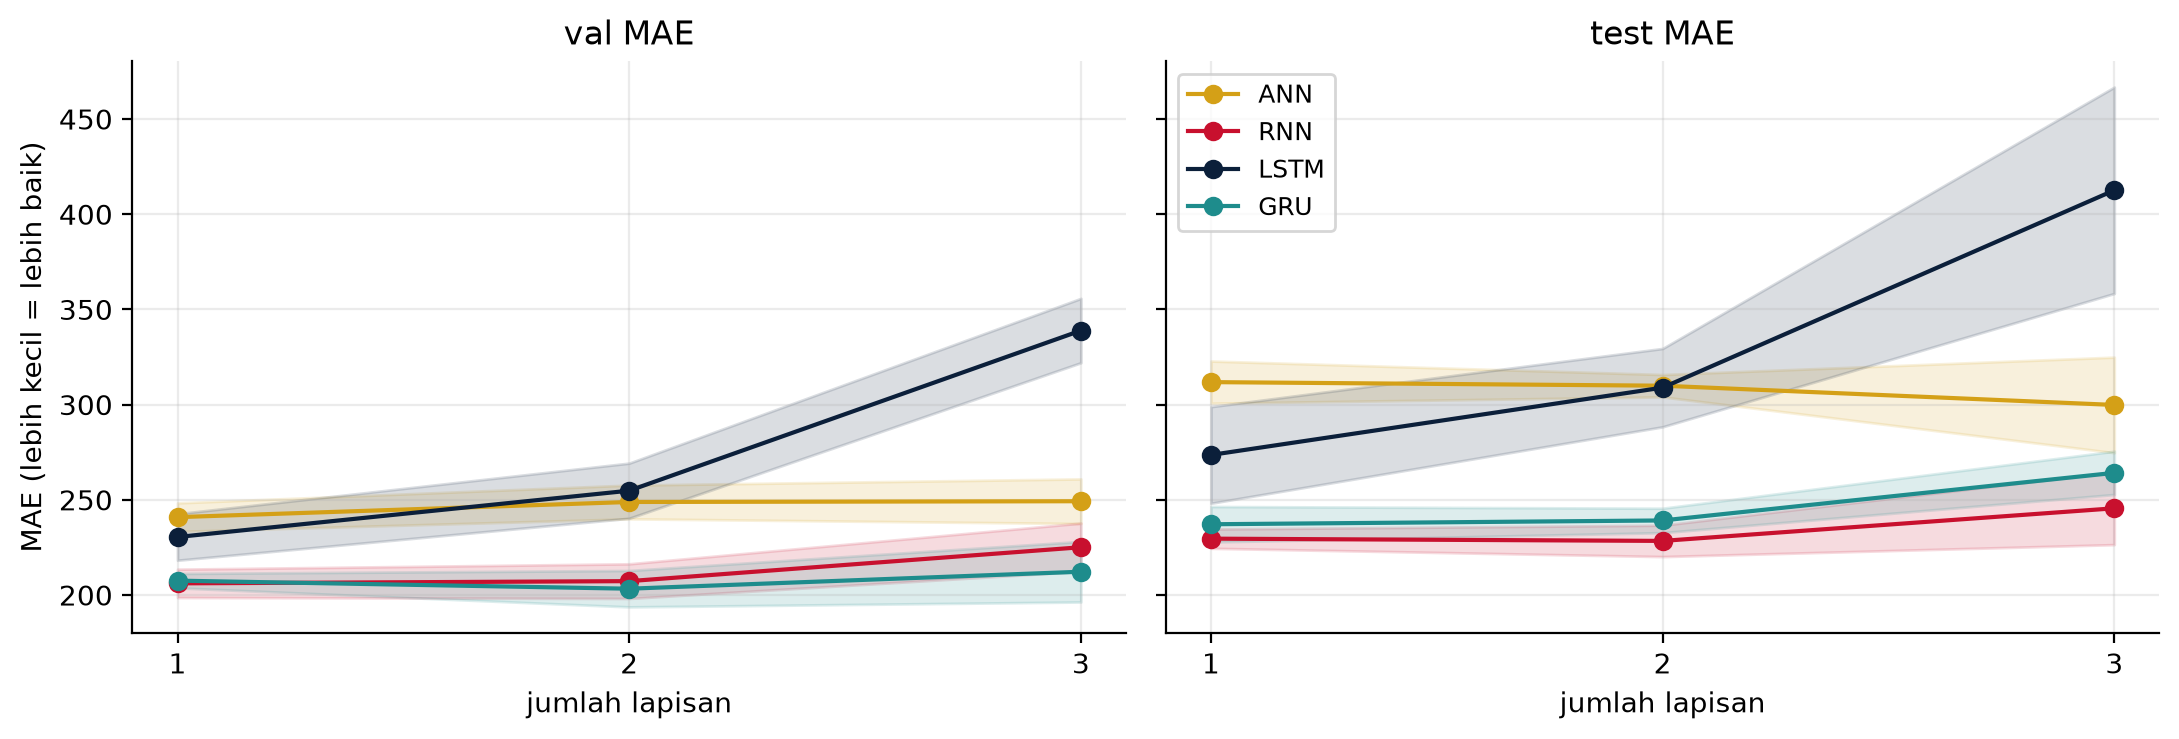
\includegraphics[width=\linewidth]{hasil/A3_layers.png}
    \caption{Pengaruh jumlah lapisan terhadap MAE validasi dan pengujian.}
    \label{fig:a3}
\end{figure}

Berdasarkan Gambar~\ref{fig:a3}, penambahan jumlah lapisan memberikan pengaruh yang berbeda pada setiap model. ANN menunjukkan MAE validasi yang relatif stabil, sedangkan RNN mengalami peningkatan MAE pada 3 lapisan. LSTM menunjukkan peningkatan MAE yang cukup besar ketika jumlah lapisan bertambah, terutama pada data pengujian. GRU juga mengalami peningkatan MAE pengujian pada 3 lapisan. Hasil ini menunjukkan bahwa model yang lebih dalam tidak selalu menghasilkan prediksi yang lebih akurat. Oleh karena itu, jumlah lapisan perlu dipilih berdasarkan hasil evaluasi setiap model.
\subsubsection{A4: Laju Pembelajaran}
Pengujian A4 dilakukan menggunakan laju pembelajaran 0.0001, 0.001, dan 0.01 untuk mengetahui pengaruhnya terhadap kinerja setiap model.

\begin{figure}[t]
    \centering
    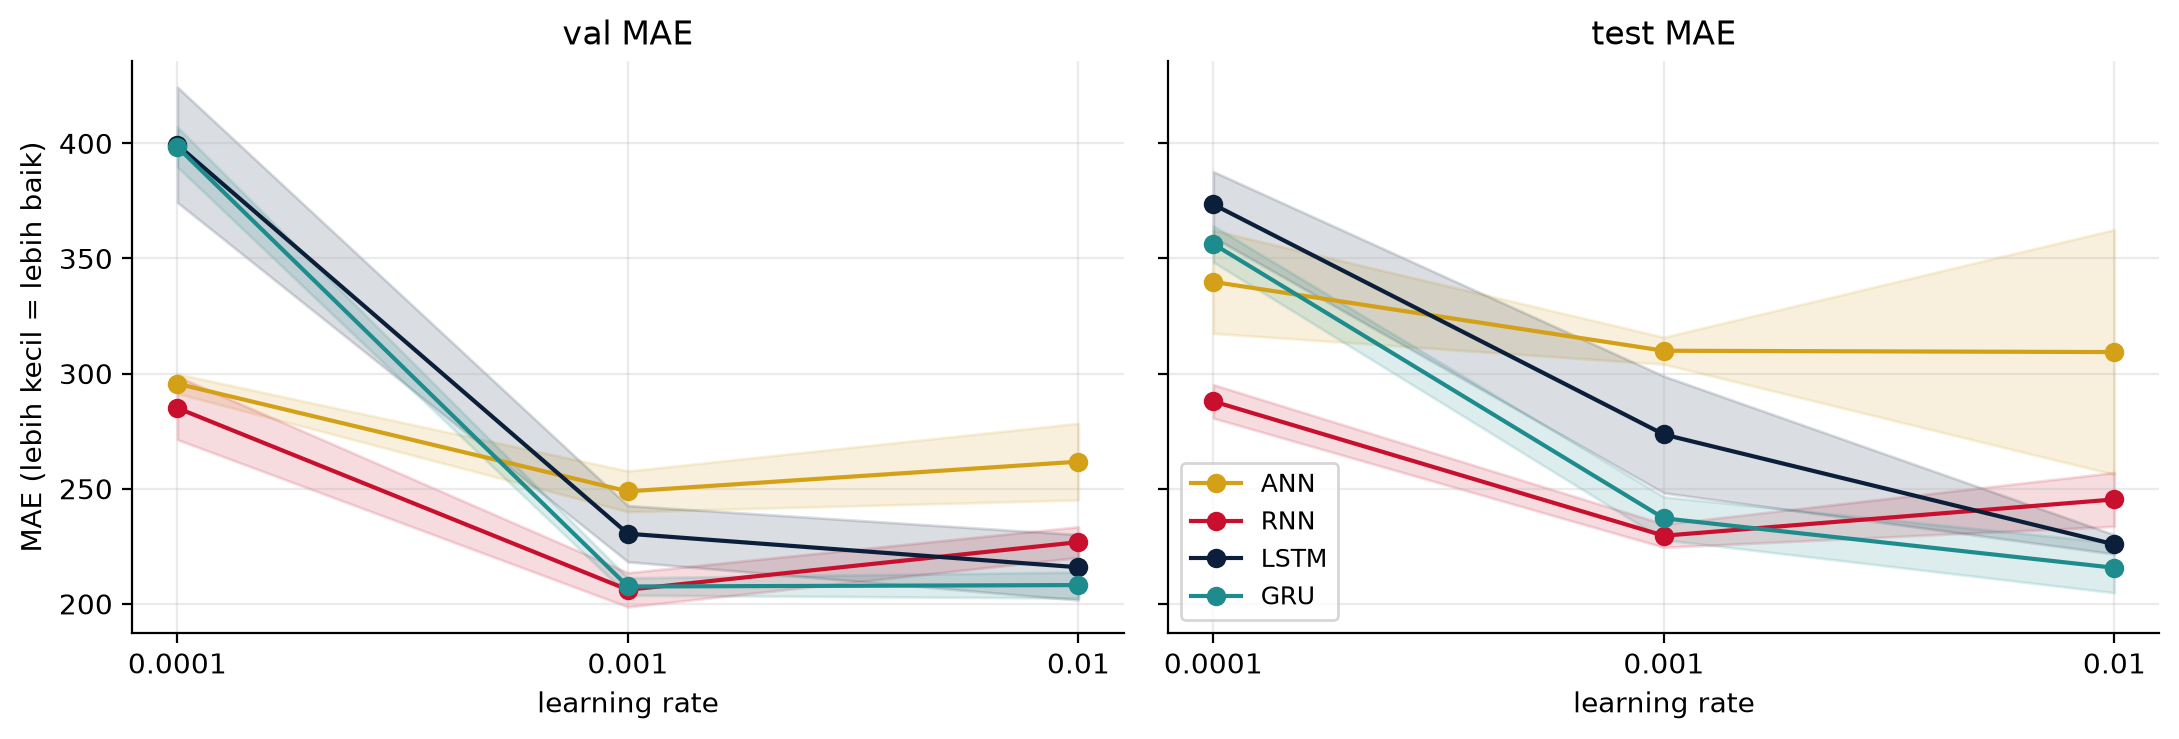
\includegraphics[width=\linewidth]{hasil/A4_lr.png}
    \caption{Pengaruh laju pembelajaran terhadap MAE validasi dan pengujian.}
    \label{fig:a4}
\end{figure}

Berdasarkan Gambar~\ref{fig:a4}, perubahan laju pembelajaran memberikan pengaruh terhadap nilai MAE setiap model. Pada data validasi, RNN, LSTM, dan GRU mengalami penurunan MAE yang cukup besar ketika laju pembelajaran meningkat dari 0.0001 menjadi 0.001. Sementara itu, ANN memiliki MAE yang lebih tinggi dibandingkan model lainnya. Pada data pengujian, RNN menghasilkan MAE terendah pada laju pembelajaran 0.001, sedangkan GRU menghasilkan MAE terendah pada laju pembelajaran 0.01. Hasil ini menunjukkan bahwa laju pembelajaran yang sesuai dapat membantu meningkatkan akurasi prediksi, tetapi pengaruhnya berbeda pada setiap model.
\subsubsection{A5: Kombinasi Fitur Masukan}

Pengujian A5 dilakukan menggunakan empat kelompok fitur masukan, yaitu net, net+call+sms, net+waktu, dan semua fitur, untuk mengetahui pengaruh kombinasi fitur terhadap kinerja prediksi trafik seluler.

\begin{figure}[t]
    \centering
    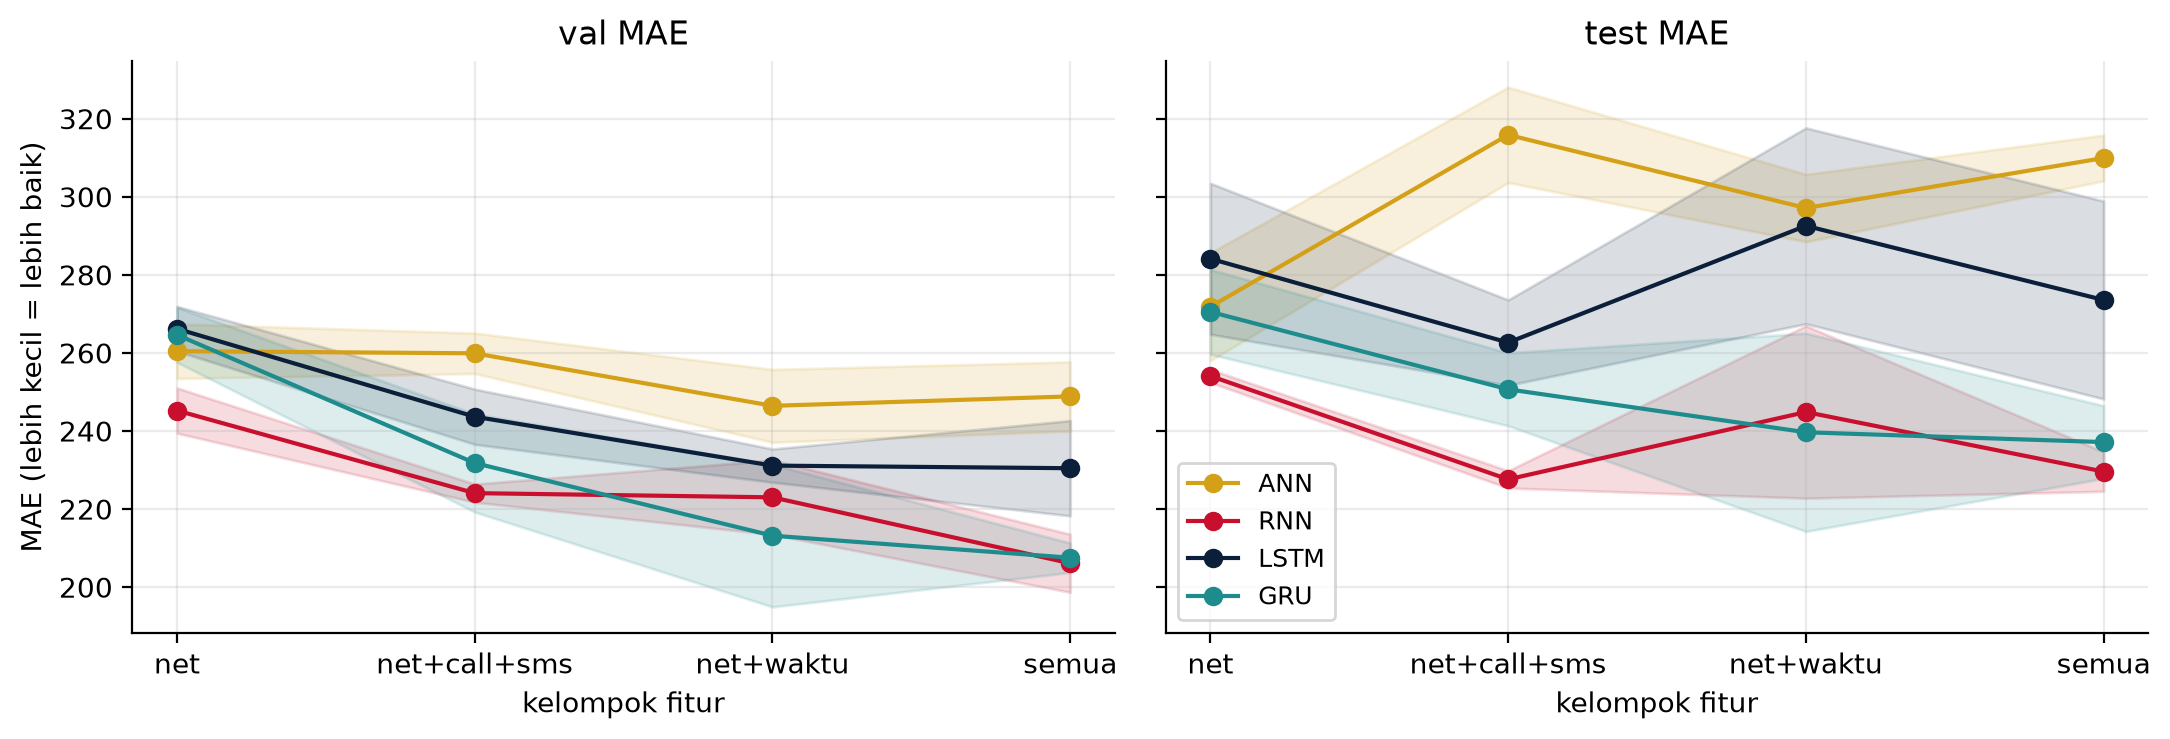
\includegraphics[width=\linewidth]{hasil/A5_fitur.png}
    \caption{Pengaruh kombinasi fitur masukan terhadap MAE validasi dan pengujian.}
    \label{fig:a5}
\end{figure}

Berdasarkan Gambar~\ref{fig:a5}, kombinasi fitur masukan memberikan pengaruh yang berbeda terhadap kinerja setiap model. Pada data validasi, RNN menunjukkan MAE yang rendah pada kombinasi fitur net+waktu, sedangkan GRU menghasilkan MAE terendah pada kombinasi fitur yang sama. Pada data pengujian, RNN menghasilkan MAE terendah pada kombinasi net+call+sms, sementara GRU menghasilkan MAE terendah pada kombinasi semua fitur. ANN cenderung memiliki MAE lebih tinggi dibandingkan model lainnya, terutama pada data pengujian. Hasil ini menunjukkan bahwa penambahan fitur tidak selalu meningkatkan akurasi prediksi, sehingga kombinasi fitur perlu dipilih berdasarkan hasil evaluasi model.

% ... analisis A5 selesai di sini

% Tabel hasil A1
\begin{table}[t]
  \centering
  \caption{Pengaruh panjang jendela $W$ terhadap test MAE (rata-rata $\pm$ simpangan baku, 3 seed).}
  \label{tab:a1}
  \begin{tabular}{@{}lcccc@{}}
    \toprule
    $W$ (jam) & ANN & RNN & LSTM & GRU \\
    \midrule
    6   & $270.71 \pm 14.58$ & $228.57 \pm 5.36$ & $276.35 \pm 14.73$ & $249.82 \pm 1.39$ \\
    24  & $309.93 \pm 5.86$ & $\mathbf{229.60 \pm 5.05}$ & $273.56 \pm 25.36$ & $237.16 \pm 9.32$ \\
    168 & $402.04 \pm 12.51$ & $\mathbf{233.51 \pm 4.83}$ & $292.82 \pm 19.95$ & $\mathbf{237.16 \pm 10.57}$ \\
    \bottomrule
  \end{tabular}
\end{table}

\subsection{Ablasi Pilihan}
\subsubsection{B1: Ukuran Batch}
Pada pengujian B1, ukuran batch yang digunakan adalah 16, 64, dan 256. Pengujian ini dilakukan untuk mengetahui pengaruh ukuran batch terhadap kinerja model prediksi trafik seluler. Hipotesis awalnya adalah ukuran batch yang lebih kecil dapat membantu model mempelajari pola data dengan lebih baik. Hasil pengujian dibandingkan berdasarkan nilai MAE validasi untuk mengetahui ukuran batch yang memberikan kinerja terbaik.

Berdasarkan hasil pengujian, ukuran batch 16 menghasilkan MAE validasi terendah pada seluruh model. Nilai MAE validasi rata-rata untuk ANN, RNN, LSTM, dan GRU masing-masing sebesar 244.40, 202.44, 209.24, dan 202.33. Ketika ukuran batch dinaikkan menjadi 64 dan 256, MAE cenderung meningkat. Dengan demikian, hipotesis bahwa ukuran batch yang lebih kecil dapat meningkatkan kinerja model didukung oleh hasil pengujian ini.


\subsubsection{B2: Dropout}
Pada pengujian B2, nilai dropout yang digunakan adalah 0, 0.2, dan 0.5. Pengujian ini bertujuan untuk mengetahui pengaruh dropout terhadap kemampuan model dalam melakukan prediksi. Hipotesis awalnya adalah penggunaan dropout dapat mengurangi overfitting dan meningkatkan kemampuan generalisasi model. Hasil pengujian dibandingkan berdasarkan nilai MAE validasi untuk mengetahui apakah penggunaan dropout memberikan peningkatan kinerja.

Hasil pengujian menunjukkan bahwa nilai dropout terbaik berbeda pada setiap model. ANN dan RNN menghasilkan MAE validasi terendah pada dropout 0, sedangkan LSTM menghasilkan MAE terendah pada dropout 0 dan GRU pada dropout 0.2. Penggunaan dropout 0.5 meningkatkan MAE pada seluruh model. Dengan demikian, hipotesis bahwa penggunaan dropout selalu meningkatkan kemampuan generalisasi tidak sepenuhnya terbukti. Pengaruh dropout bergantung pada karakteristik model yang digunakan.
\subsection{Ablasi Pilihan}

\subsection{Konfigurasi Terbaik}
Konfigurasi terbaik setiap model dipilih berdasarkan nilai MAE validasi terendah. Hasil pengujian menunjukkan bahwa model ANN memperoleh MAE validasi sebesar 212,3, RNN sebesar 200,1, LSTM sebesar 207,1, dan GRU sebesar 188,7. Dengan demikian, GRU menjadi model dengan kinerja terbaik berdasarkan MAE validasi.

Pada data minggu pengujian, konfigurasi terbaik menghasilkan MAE sebesar 270,7 untuk ANN, 224,5 untuk RNN, 245,6 untuk LSTM, dan 220,3 untuk GRU. Seluruh model terbaik menghasilkan MAE lebih rendah dibandingkan konfigurasi acuannya. GRU memperoleh MAE test terendah, yaitu 220,3.

Pada pengujian Natal, MAE yang diperoleh adalah 531,6 untuk ANN, 404,5 untuk RNN, 491,1 untuk LSTM, dan 435,2 untuk GRU. Hasil ini menunjukkan bahwa model terbaik pada minggu pengujian belum tentu menjadi model terbaik pada periode Natal. RNN menghasilkan MAE Natal terendah, yaitu 404,5, sehingga kinerja model dapat berbeda bergantung pada periode pengujian.
\subsection{Uji Generalisasi}
Pengujian generalisasi dilakukan dengan membandingkan konfigurasi acuan dan konfigurasi terbaik pada data pengujian. Hasil menunjukkan bahwa konfigurasi terbaik tidak selalu menghasilkan MAE yang lebih rendah pada semua model. Pada ANN, MAE test turun dari 222,3 menjadi 213,9. Pada GRU, MAE turun dari 190,8 menjadi 188,4, sedangkan pada LSTM turun dari 247,3 menjadi 243,8. Namun, pada RNN, MAE meningkat dari 193,0 menjadi 204,2.

Pada pengujian periode Natal, MAE konfigurasi terbaik meningkat pada ANN dan GRU, masing-masing menjadi 688,7 dan 620,8. Sebaliknya, MAE LSTM turun dari 950,8 menjadi 839,5, sedangkan RNN meningkat dari 534,7 menjadi 548,8. Hal ini menunjukkan bahwa konfigurasi terbaik pada data sebelumnya belum tentu memberikan hasil terbaik pada periode yang berbeda. Perubahan pola trafik dapat menjadi salah satu faktor yang memengaruhi kemampuan generalisasi model.
% ---------------------------------------------------------------------
\section{Pembahasan}
Hasil pengujian menunjukkan bahwa kinerja model dipengaruhi oleh pemilihan hyperparameter dan jenis arsitektur yang digunakan. Pada ablasi panjang jendela, penambahan jumlah data masukan tidak selalu meningkatkan akurasi prediksi. Hal ini dapat terjadi karena jendela yang lebih panjang membuat model harus mempelajari pola yang lebih kompleks. Oleh karena itu, panjang jendela perlu disesuaikan dengan karakteristik data trafik.

Ukuran hidden, jumlah lapisan, laju pembelajaran, dan kombinasi fitur juga memengaruhi hasil prediksi. Penambahan jumlah neuron atau lapisan tidak selalu menghasilkan MAE yang lebih rendah karena model yang lebih kompleks belum tentu dapat mempelajari pola data dengan lebih baik. Laju pembelajaran yang sesuai membantu proses pelatihan mencapai hasil yang lebih baik, sedangkan pemilihan fitur masukan menentukan informasi yang dapat dimanfaatkan model untuk melakukan prediksi.

Perbedaan kinerja antar-model menunjukkan bahwa setiap arsitektur memiliki kemampuan yang berbeda dalam mempelajari pola trafik. Model GRU memperoleh MAE validasi terendah pada hasil konfigurasi terbaik, sedangkan pada pengujian periode Natal, RNN menghasilkan MAE terendah berdasarkan hasil yang telah dibahas sebelumnya. Perubahan ini menunjukkan bahwa model dengan kinerja terbaik pada satu periode belum tentu memberikan hasil terbaik pada periode lain. Perbedaan pola trafik ant periode dapat memengaruhi kemampuan model dalam melakukan generalisasi.

Penelitian ini memiliki beberapa keterbatasan. Pengujian dilakukan pada satu kota, menggunakan data pelatihan selama empat minggu, dan satu kali pembagian data berdasarkan waktu. Selain itu, hasil dari tiga seed perlu dibandingkan untuk mengetahui kestabilan model. Oleh karena itu, penelitian selanjutnya dapat menggunakan data dari lebih banyak lokasi, periode pelatihan yang lebih panjang, dan beberapa pembagian waktu untuk memperoleh hasil evaluasi yang lebih kuat.

% ---------------------------------------------------------------------
\section{Kesimpulan}
Berdasarkan hasil pengujian, pemilihan hyperparameter dan arsitektur model memengaruhi kinerja prediksi trafik jaringan. Model GRU memperoleh MAE validasi terendah sebesar 188,7, sedangkan pada pengujian minggu, GRU menghasilkan MAE sebesar 220,3. Pada periode Natal, RNN memberikan hasil terbaik dengan MAE sebesar 404,5, yang menunjukkan bahwa kinerja model dapat berubah pada periode pengujian yang berbeda. Dengan demikian, pemilihan model tidak cukup hanya berdasarkan hasil validasi, tetapi juga perlu mempertimbangkan kemampuan generalisasi terhadap perubahan pola trafik.

% ---------------------------------------------------------------------
\section*{Kontribusi Anggota}
\begin{tabular}{@{}lp{0.62\linewidth}@{}}
  Vaulina Fatrisia Siburian & Pengerjaan ablasi wajib A1--A3, ablasi pilihan B1, dan analisis hasil pengujian. \\
  Ashintya Linsih Nainggolan & Pengerjaan ablasi wajib A4--A5, ablasi pilihan B2, konfigurasi terbaik, uji generalisasi, pembahasan, dan kesimpulan. \\
\end{tabular}

% ---------------------------------------------------------------------
\section*{Pernyataan Penggunaan AI}
ChatGPT digunakan untuk membantu merapikan penulisan laporan, menyusun analisis hasil pengujian, dan memperbaiki format penulisan LaTeX. Seluruh angka dan hasil pengujian mengacu pada data eksperimen yang dilakukan oleh kelompok.

\section*{Kode dan Data}
Kode, notebook beserta output, dan seluruh hasil run tersedia di \url{https://github.com/vaulina124400011-spec/prediksi-trafik-jaringan}.

\bibliographystyle{IEEEtran}
\bibliography{references}

\end{document}
